\begin{appendix}

\chapter{ Anexo: Certificación de software de la raspberry}
\begin{figure}[H]
    \centering
    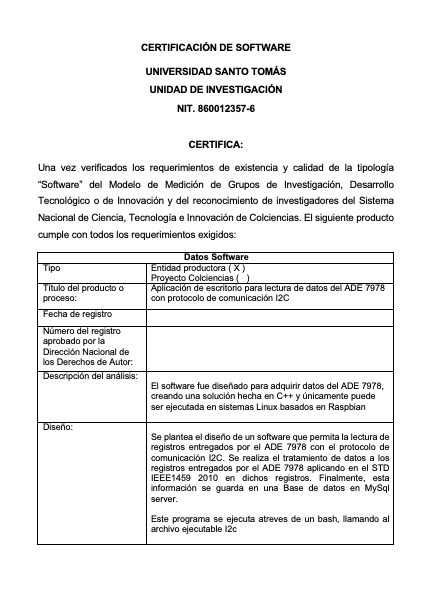
\includegraphics[width = 14cm]{Anexos/raspberry-1.png}
    \label{fig:raspberry1}
\end{figure}
\begin{figure}[H]
    \centering
    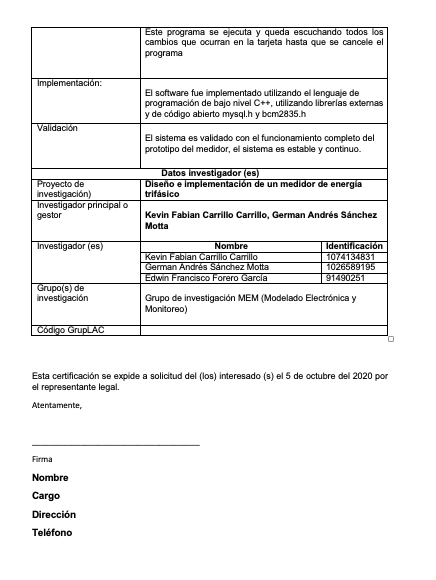
\includegraphics[width = 14cm]{Anexos/raspberry-2.png}
    \caption{Certificación de software raspberry} 
    \label{fig:raspberry2}
\end{figure}

\chapter{ Anexo: Certificación de software del servicio web(API)}
\begin{figure}[H]
    \centering
    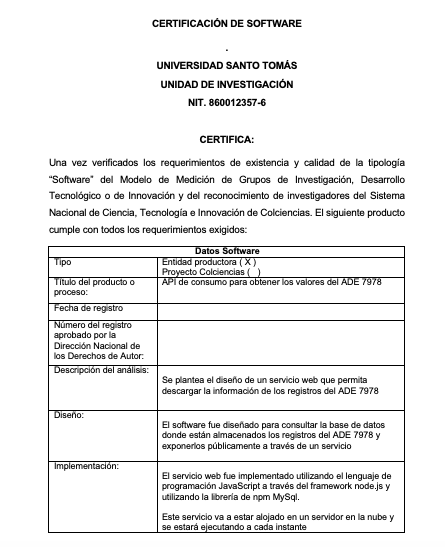
\includegraphics[width = 14cm]{Anexos/api-1.png}
    \label{fig:api1}
\end{figure}
\begin{figure}[H]
    \centering
    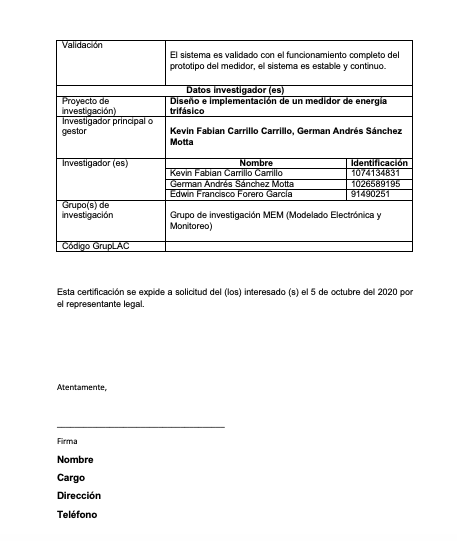
\includegraphics[width = 14cm]{Anexos/api-2.png}
    \caption{Certificación de software del servicio web} 
    \label{fig:api2}
\end{figure}

\chapter{ Anexo: Certificación de software de la página web}
\begin{figure}[H]
    \centering
    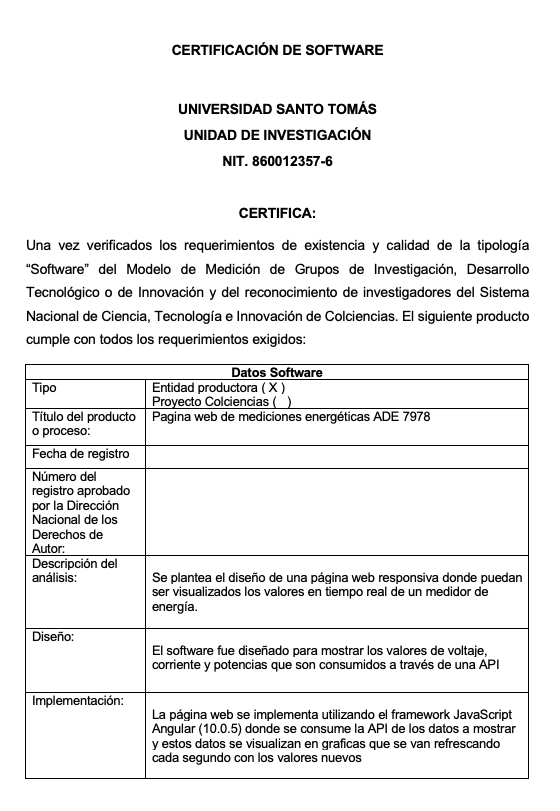
\includegraphics[width = 12cm]{Anexos/front-1.png}
    \label{fig:front1}
\end{figure}
\begin{figure}[H]
    \centering
    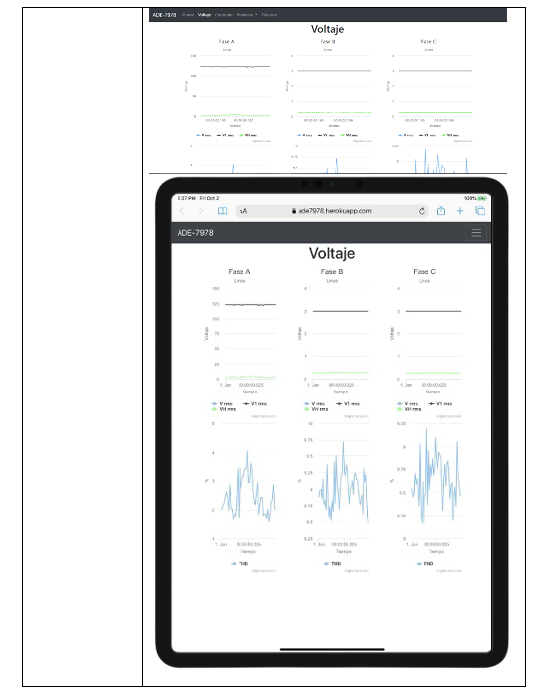
\includegraphics[width = 14cm]{Anexos/front-2.png}
    \label{fig:front2}
\end{figure}
\begin{figure}[H]
    \centering
    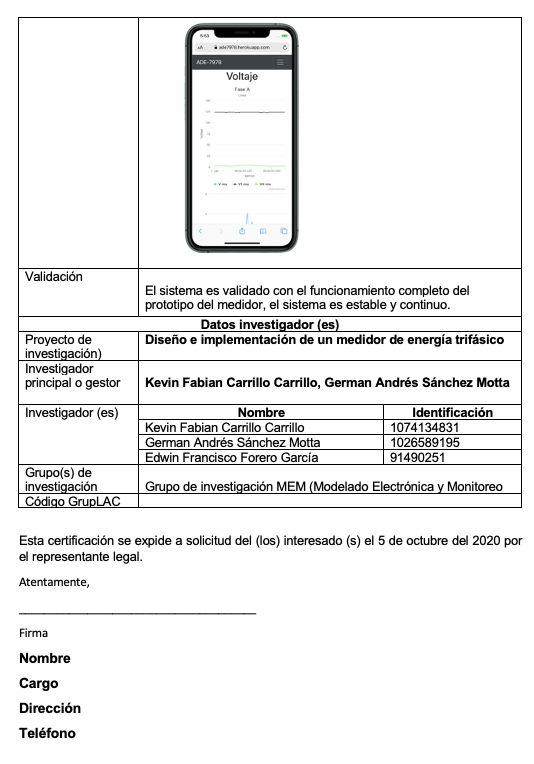
\includegraphics[width = 14cm]{Anexos/front-3.png}
    \caption{Certificación de software de la página web} 
    \label{fig:front3}
\end{figure}

% \chapter{Anexo: Nombrar el anexo B de acuerdo con su contenido}
% MANEJO DE LA BIBLIOGRAF\'{I}A: la bibliograf\'{\i}a es la relaci\'{o}n de las fuentes documentales consultadas por el investigador para sustentar sus trabajos. Su inclusi\'{o}n es obligatoria en todo trabajo de investigaci\'{o}n. Cada referencia bibliogr\'{a}fica se inicia contra el margen izquierdo.\\

% La NTC 5613 establece los requisitos para la presentaci\'{o}n de referencias bibliogr\'{a}ficas citas y notas de pie de p\'{a}gina. Sin embargo, se tiene la libertad de usar cualquier norma bibliogr\'{a}fica de acuerdo con lo acostumbrado por cada disciplina del conocimiento. En esta medida es necesario que la norma seleccionada se aplique con rigurosidad.\\

% Es necesario tener en cuenta que la norma ISO 690:1987 (en Espa\~{n}a, UNE 50-104-94) es el marco internacional que da las pautas m\'{\i}nimas para las citas bibliogr\'{a}ficas de documentos impresos y publicados. A continuaci\'{o}n se lista algunas instituciones que brindan par\'{a}metros para el manejo de las referencias bibliogr\'{a}ficas:\\

% \begin{center}
% \centering%
% \begin{tabular}{|p {7.5 cm}|p {7.5 cm}|}\hline
% \arr{Instituci\'{o}n}&Disciplina de aplicaci\'{o}n\\\hline%
% Modern Language Association (MLA)&Literatura, artes y humanidades\\\hline%
% American Psychological Association (APA)&Ambito de la salud (psicolog\'{\i}a, medicina) y en general en todas las ciencias sociales\\\hline
% Universidad de Chicago/Turabian &Periodismo, historia y humanidades.\\\hline
% AMA (Asociaci\'{o}n M\'{e}dica de los Estados Unidos)&Ambito de la salud (psicolog\'{\i}a, medicina)\\\hline
% Vancouver &Todas las disciplinas\\\hline
% Council of Science Editors (CSE)&En la actualidad abarca diversas ciencias\\\hline
% National Library of Medicine (NLM) (Biblioteca Nacional de Medicina)&En el \'{a}mbito m\'{e}dico y, por extensi\'{o}n, en ciencias.\\\hline
% Harvard System of Referencing Guide &Todas las disciplinas\\\hline
% JabRef y KBibTeX &Todas las disciplinas\\\hline
% \end{tabular}
% \end{center}

% Para incluir las referencias dentro del texto y realizar lista de la bibliograf\'{\i}a en la respectiva secci\'{o}n, puede utilizar las herramientas que Latex suministra o, revisar el instructivo desarrollado por el Sistema de Bibliotecas de la Universidad Nacional de Colombia\footnote{Ver: www.sinab.unal.edu.co}, disponible en la secci\'{o}n "Servicios", opci\'{o}n "Tr\'{a}mites" y enlace "Entrega de tesis".

\end{appendix}